% -------------------------------------------------------------------------------- %

\begin{exercise}[\textbf{Missing information}]

An investigation of ethnic differences in reports of pain perception
was presented at the annual meeting of the American Psychosomatic Society
(Mar. 2001). A sample of 55 blacks and 159 whites participated in the study.
Subjects rated (on a 13-point scale) the intensity and unpleasantness of
pain felt when a bag of ice was placed on their foreheads for two minutes.
(Higher ratings correspond to higher pain intensity.)
A summary of the results is provided in the following table.

\begin{center}
    \begin{tabular}{c|cc}
        & Blacks & Whites \\
        \hline
        Sample Size & 55 & 159 \\
        Mean pain intensity & 8.2 & 6.9
    \end{tabular}
\end{center}

\begin{enumerate}[label = (\alph*)]
    \item Why is it dangerous to draw a statistical inference from the summarized data? Explain.
    \item What values of the missing sample standard deviations would lead
    you to conclude (at $\alpha = 0.05$) that blacks, on average, have
    a higher pain intensity rating than whites?
    \item What values of the missing sample standard deviation would lead
    you to an inconclusive decision (at $\alpha = 0.05$) regarding whether
    blacks or whites have a higher mean intensity rating?
\end{enumerate}

\end{exercise}

% -------------------------------------------------------------------------------- %

\begin{solution}

Inferences from the given summarized data are dangerous, since the missing
information, the sample variance, plays a crucial role in the calculation
of confidence intervals or p-values. Different values of the missing variance
could skew the results in either direction.

Let's calculate the 95\%-confidence interval 
as a function of the missing sample standard deviations.

\begin{align*}
    8.2 - 6.9 \pm z_{\alpha/2}\sqrt{\frac{s_1^2}{n_1} + \frac{s_2^2}{n_2}}
    \approx  1.3 \pm 1.959964 \cdot \sqrt{\frac{s_1^2}{55} + \frac{s_2^2}{159}}.
\end{align*}

Therefore we would conclude a higher pain intensity for blacks if

\begin{align*}
    \sqrt{\frac{s_1^2}{55} + \frac{s_2^2}{159}} < \frac{1.3}{1.959964},
\end{align*}

i.e., if the values $(s_1,s_2)$ lie within the blue ellipse below.

\begin{figure}[H]
    \centering
    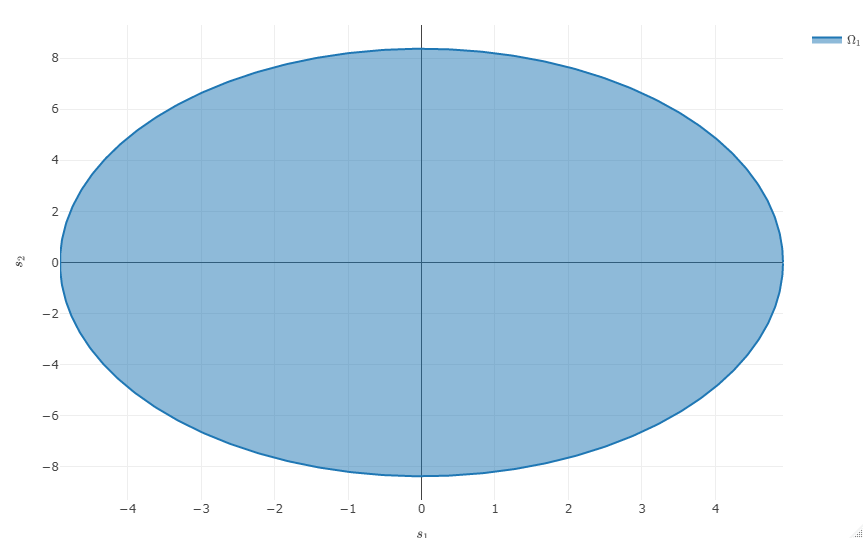
\includegraphics[width = 0.8 \textwidth]{12.3.png}
\end{figure}

If the values for $(s_1,s_2)$ lie outside of the ellipse, this implies
that $0$ is part of our 95\%-confidence interval and we are lead to
an inconclusive decision.

\end{solution}

% -------------------------------------------------------------------------------- %
